\section{Potential Sources of Error}
\label{sec:error}

Let us collate the assumptions of classical theories for calculation of rate constants using the definitions from section 2.1:

\begin{itemize}
\item[1.] the motion of electrons and nuclei can be separated (accordingly to the Born-Oppenheimer approximation),
\item[2.] the motion of nuclei can be described by classical mechanics,
\item[3.] the distribution of phase points within a selected box is in equilibrium,
\item[4.] the trajectories entering a box are statistically independent of the trajectories leaving the box,
\item[5.] \begin{itemize} 
\item[a)] the population in each box i is in equilibrium with every other box j,
\item[b)] the distribution of FPT's is strictly exponential,
\item[c)] the distribution of FPT's is a non-increasing continuous function.
\end{itemize}
\end{itemize}
Both the method of reactive flux and the MFPT based method presented in this work require assumptions 1-4 to be valid.
Assumption 5.b) is a weaker form of assumption 5.a) and is required by equilibrium flux methods.
An even weaker assumption, 5.c) is required by the MFPT approach used here.
An FPT-BXD simulation protocol that correctly reproduces classical dynamics cannot be in conflict with assumptions 3, 4 and 5 and the sampling must be ergodic.

The inversion procedure used by Glowacki {\it et al.}\cite{Glowacki2009} can sometimes give incorrect equilibrium distributions.
If the potential energy gradient points towards the box boundary, BXD trajectories moving almost tangentially to the dividing surface cannot leave the neighbourhood of the boundary because they are reflected from the boundary at the same small angle.
Such trajectories will unphysically increase the probability of states close to the boundary and therefore increase the calculated flux.
To allow sampling of trajectories that penetrate deeper into the box, the velocity directions of all particles should be randomised. 
A new inversion method is tested  in the present work.

As discussed in section 2.4, BXD simulations in both neighbouring boxes A and B are necessary to calculate the rate constant corresponding to transitions from A to B.
The sum of the MFPT's has to be divided into boxes according to the equilibrium fluxes (\ref{eq:corrected}).
However, without internal barriers the uncorrected and corrected rate constants can be almost equal.
Since the ratio of equilibrium fluxes calculated from simulations can be inaccurate, the correction can be omitted if the recrossing error dominates.
Such a simplification must be checked by plotting the distribution of lag times.


If the configuration space is divided into two boxes representing the species only, the rate constant calculated by fitting $P(t)$ obtained from equation (\ref{eq:pt-exp}) and scaled by equilibrium fluxes using equation (\ref{eq:pt-exp}) gives in principle the exact classical rate constant for the system.
However, the efficiency gain of BXD is based on the possibility of introducing new boxes.
Division of the space into more boxes results in less assigned volume per box and therefore smaller distances between the box boundaries.
An insufficient distance between two neighbouring boxes can cause the incoming trajectories to be correlated with trajectories leaving the box.
The decorrelation is one of the requirements of MSM's (assumption 4 above) and can be mathematically formulated as
\begin{equation}
\label{eq:decorrelation}
k_{\rm i \rightarrow j \rightarrow k} = k_{\rm l \rightarrow j \rightarrow k} ~,
\end{equation}
where i, k, l are boxes neighbouring box j and $k_{\rm i \rightarrow j \rightarrow k}$ is the rate constant $k_{\rm j \rightarrow k}$ under the constraint that trajectories can enter box j  only from box i.
The condition can be written as
\begin{equation}
\label{eq:decorr-mfpt}
{\rm MFPT}_{\rm \partial ij \rightarrow \partial jk} = {\rm MFPT}_{\rm \partial lj \rightarrow \partial jk} ~.
\end{equation}
Here ${\rm MFPT}_{\rm \partial ij \rightarrow \partial jk}$ is the mean first passage time of those trajectories exiting box j through dividing surface ${\rm \partial jk}$, which entered box j through dividing surface ${\rm \partial ij}$.
Such data can easily be obtained from FTP-BXD simulations by recording the endpoints and evolution times of all subtrajectories.
This procedure was not possible with the old formula in which recrossing and the equality of weight of long and short trajectories in the summation would cause recrossing to artificially decrease the ${\rm MFPT}_{\rm \partial kj \rightarrow \partial jk}$ compared to other ${\rm MFPT}_{\rm \partial ij \rightarrow \partial jk}$.
Analysis of the correlation in the simulation can indicate that the box is too small (${\rm MFPT}_{\rm \partial ij \rightarrow \partial jk} < {\rm MFPT}_{\rm \partial kj \rightarrow \partial jk}$) or that the box contains a high internal barrier (${\rm MFPT}_{\rm \partial kj \rightarrow \partial jk} < {\rm MFPT}_{\rm \partial ij \rightarrow \partial jk}$).

Even if ${\rm MFPT}_{\rm \partial kj \rightarrow \partial jk} = {\rm MFPT}_{\rm \partial ij \rightarrow \partial jk}$, the Markovian assumption can be broken by an inappropriate configuration of boxes. 
A high internal barrier could spread throughout more boxes (see figure \ref{fig:bar-3-boxy}). 
However, such cases will probably not be commonplace.
\begin{figure}[h]
\centering
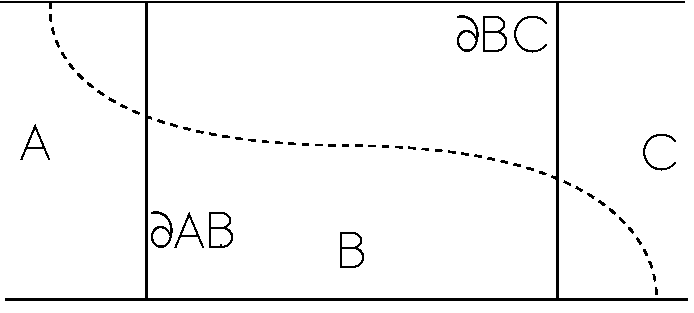
\includegraphics[width=8cm]{Images/manyboxcorrelation.pdf}
\caption[Multi-box correlation]{Illustration of the correlation error arising from an internal barrier (dashed line) spread over more boxes. In spite of the fact that no correlation can be implied from a BXD simulation in box B, the transition from box A to box C will be much smaller than calculated from a BXD simulation ($\rm MFPT_{A \rightarrow C} > MFPT_{A \rightarrow B} + MFPT_{B \rightarrow C}$), so assumption 4 is violated. The method proposed in this section cannot identify such a pathological case.}
\label{fig:bar-3-boxy}
\end{figure}


